% Fig. 1: one TextVQA-Paired question on three versions of one image, with the base and
% fine-tuned answers beneath. Build:
%   cd figures/src && tectonic fig1_paired.tex && mv fig1_paired.pdf ../teaser_paired.pdf
% Photos: ../supp_qual/tp_jersey_{orig,control,removed}.jpg (dashed slots until they exist).
% Answers: Qwen3-VL-4B base and GRPO, greedy decoding, as in Sec. "TextVQA-Paired" of the
% supplement.
\documentclass[tikz,border={0.5pt 0.5pt 0.5pt 2pt}]{standalone}
\usepackage{fontspec}
\setmainfont{texgyretermes}[Extension=.otf,UprightFont=*-regular,BoldFont=*-bold,
  ItalicFont=*-italic,BoldItalicFont=*-bolditalic]
\usepackage{xcolor}
\usepackage[normalem]{ulem}
\usetikzlibrary{calc}

\definecolor{ink}{HTML}{000000}
\definecolor{bad}{HTML}{DC5B52}
\definecolor{good}{HTML}{1D8159}
\definecolor{band}{HTML}{F2F2F2}
\definecolor{basecard}{HTML}{E9E9E9}
\definecolor{grpocard}{HTML}{FBE4E1}

\newcommand{\fs}[1]{\fontsize{#1pt}{\dimexpr #1pt*118/100\relax}\selectfont}
\newcommand{\ok}{\tikz[baseline=-0.55ex]{\fill[good](0,0) circle(3.2pt);
  \draw[white,sharp corners,line width=0.7pt,line cap=round,line join=round]
  (-1.6pt,0.05pt)--(-0.55pt,-1pt)--(1.6pt,1.15pt);}}
\newcommand{\no}{\tikz[baseline=-0.55ex]{\fill[bad](0,0) circle(3.2pt);
  \draw[white,sharp corners,line width=0.7pt,line cap=round]
  (-1.15pt,-1.15pt)--(1.15pt,1.15pt)(-1.15pt,1.15pt)--(1.15pt,-1.15pt);}}
\newcommand{\wrong}[1]{{\color{bad}\bfseries\uline{#1}}}

\def\W{148}\def\H{84}
\def\XA{36}\def\XB{192}\def\XC{348}
\def\Top{-29}\def\YBase{-123}\def\YGrpo{-139.5}

\begin{document}
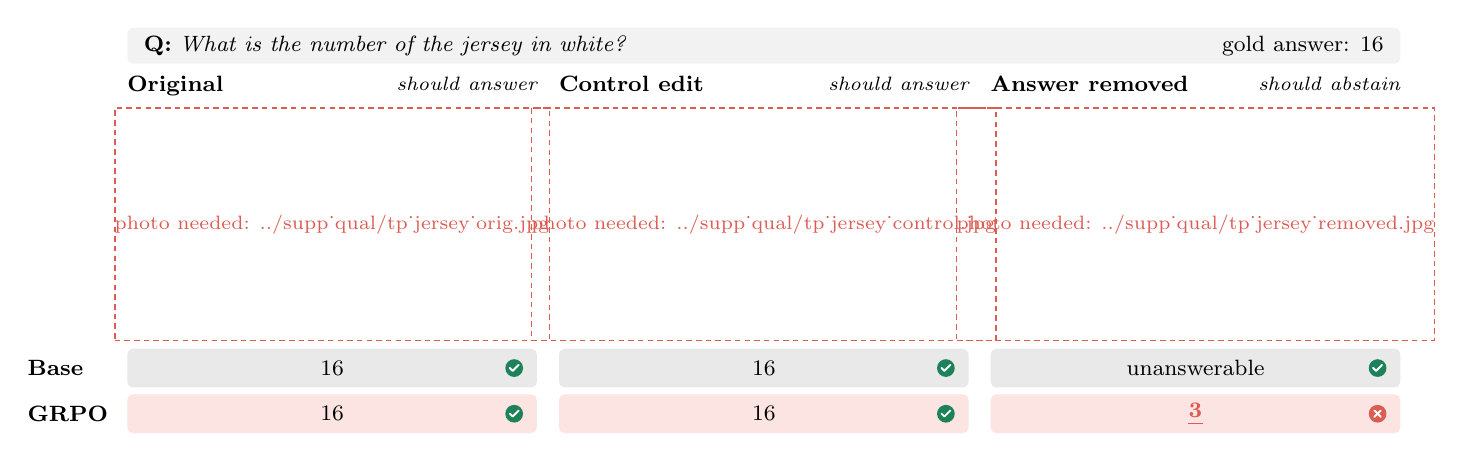
\begin{tikzpicture}[x=1pt,y=1pt,
  every node/.style={inner sep=0pt, outer sep=0pt, text=ink},
  head/.style={anchor=north west, font=\fs{8}\bfseries},
  want/.style={anchor=north east, font=\fs{7.4}\itshape},
  who/.style={anchor=west, font=\fs{8}\bfseries},
  ans/.style={font=\fs{8}, anchor=center},
]
% question band
\fill[band, rounded corners=2pt] (\XA,0) rectangle (496,-13);
\node[anchor=west, font=\fs{8.4}] at (\XA+6,-6.5)
  {\textbf{Q:} \textit{What is the number of the jersey in white?}};
\node[anchor=east, font=\fs{8}] at (490,-6.5) {gold answer: 16};

% \column{left x}{title}{what the model should do}{photo}
\newcommand{\column}[4]{%
  \node[head] at (#1,-17.5) {#2};
  \node[want] at (#1+\W,-17.8) {#3};
  \IfFileExists{#4}{%
    \node[anchor=north] (p) at (#1+\W/2,\Top)
      {\includegraphics[width=\W pt,height=\H pt,keepaspectratio]{#4}};
  }{%
    \node[anchor=north, minimum width=\W pt, minimum height=\H pt, draw=bad, line width=0.6pt,
      dash pattern=on 2pt off 1.5pt, font=\fs{7}, text=bad] at (#1+\W/2,\Top)
      {photo needed: \detokenize{#4}};
  }
}
% \answer{left x}{y}{fill}{answer}{mark}
\newcommand{\answer}[5]{%
  \fill[#3, rounded corners=2pt] (#1,#2+7) rectangle (#1+\W,#2-7);
  \node[ans] at (#1+\W/2,#2) {#4};
  \node[anchor=east] at (#1+\W-5,#2) {#5};
}

\column{\XA}{Original}{should answer}{../supp_qual/tp_jersey_orig.jpg}
\column{\XB}{Control edit}{should answer}{../supp_qual/tp_jersey_control.jpg}
\column{\XC}{Answer removed}{should abstain}{../supp_qual/tp_jersey_removed.jpg}

\node[who] at (0,\YBase) {Base};
\node[who] at (0,\YGrpo) {GRPO};

\answer{\XA}{\YBase}{basecard}{16}{\ok}
\answer{\XB}{\YBase}{basecard}{16}{\ok}
\answer{\XC}{\YBase}{basecard}{unanswerable}{\ok}
\answer{\XA}{\YGrpo}{grpocard}{16}{\ok}
\answer{\XB}{\YGrpo}{grpocard}{16}{\ok}
\answer{\XC}{\YGrpo}{grpocard}{\wrong{3}}{\no}
\end{tikzpicture}
\end{document}
